\section{Background estimation}

Table~\ref{tab:yield_prefit} sumarizes the background yields for $ZZjj \rightarrow \lllljj$ channel in 139~\ifb.
Uncertainties on the predictions include both statistical and systematic components.
"Others" includes minor contributions from non-ZZ processes including \Zjet, top-quark, triboson and ttV processes.
Detail of estimation for each source will described below.

\begin{table}[!htbp]
\sisetup{
table-number-alignment = center,
table-align-uncertainty=true
}
\begin{center}
   \begin{tabular}{
   c
   S[table-format = 3.1]@{$\,\pm\,$}
   S[table-format = 2.1]
   }
   \hline
   Process                 & \multicolumn{2}{c}{\lllljj}       \\
   \hline
   EW-$ZZjj$               &  20.6 &  2.5  \\
   QCD-\qqZZ               &  77   & 25    \\
   QCD-\ggZZ               &  13.1 &  4.4  \\
   Others                  &   3.2 &  2.1  \\
   \hline
   Total                   & 114   & 26    \\
   \hline
   Data                    &  \multicolumn{2}{l}{127}           \\
   \hline
   \end{tabular}
\end{center}
\caption{
Observed data and expected signal and background yields in 139~\ifb{} of luminosity.
Minor backgrounds are summed together as `Others'.
Uncertainties on the predictions include both statistical and systematic components.
}
\label{tab:yield_prefit}
\end{table}

\subsection{QCD backgrounds}

The QCD-ZZjj production, which include both qq and gg induced processes, is an irreducible background in the search of EW-ZZjj production.
A QCD-enriched control region (CR) is defined to constrain the contribution by reverting either the $\mjj$ or $\dyjj$ requirements:\\
	$\mjj <$ 300~\GeV{} or $\dyjj <$ 2 \\
Then the normalization factor of QCD-ZZjj process is included into statistical fit as a float parameter to properly treat the uncertainty correlations between SR and CR, 
while the shapes are taken from MC simulation.
Table~\ref{tab:yield_qcdcr} shows the event yields of each background components in this CR.
Uncertainties are statistical one only.
\begin{table}[!htbp]
\sisetup{
table-number-alignment = center,
table-align-uncertainty=true
}
\begin{center}
   \begin{tabular}{
   c
   S[table-format = 3.1]@{$\,\pm\,$}
   S[table-format = 2.1]
   }
   \hline
   Process                 & \multicolumn{2}{c}{\lllljj}       \\
   \hline
   EW $ZZjj$               &   3.9 &  0    \\
   QCD $ZZjj$              & 136.9 &  0.6  \\
   QCD $ggZZjj$            &  16.8 &  0.1  \\
   Diboson                 &   0.3 &  0.1  \\
   Triboson                &   1.6 &  0.1  \\
   \Zjet                   &   \multicolumn{2}{l}{0}    \\
   \ttbar                  &   \multicolumn{2}{l}{0}    \\
   \hline
   Total                   & 159.5 &  0.62 \\
   \hline
   Data                    &  \multicolumn{2}{l}{152}           \\
   \hline
   \end{tabular}
\end{center}
\caption{
Observed data and expected signal and background yields in 139~\ifb{} of luminosity.
Diboson includes all the other diboson processes discussed in section~\ref{sec:mc}, except those with four-lepton final state.
Uncertainties include only MC statistic.
No events from \Zjet and \ttbar MC pass the selection, and are indicated as 0 in the table.
}
\label{tab:yield_qcdcr}
\end{table}
The distributions of 4l and dijet invariant mass in QCD CR are shown in figure~\ref{fig:qcdcr_prefit}.
\begin{figure}[!htb]
  \centering
  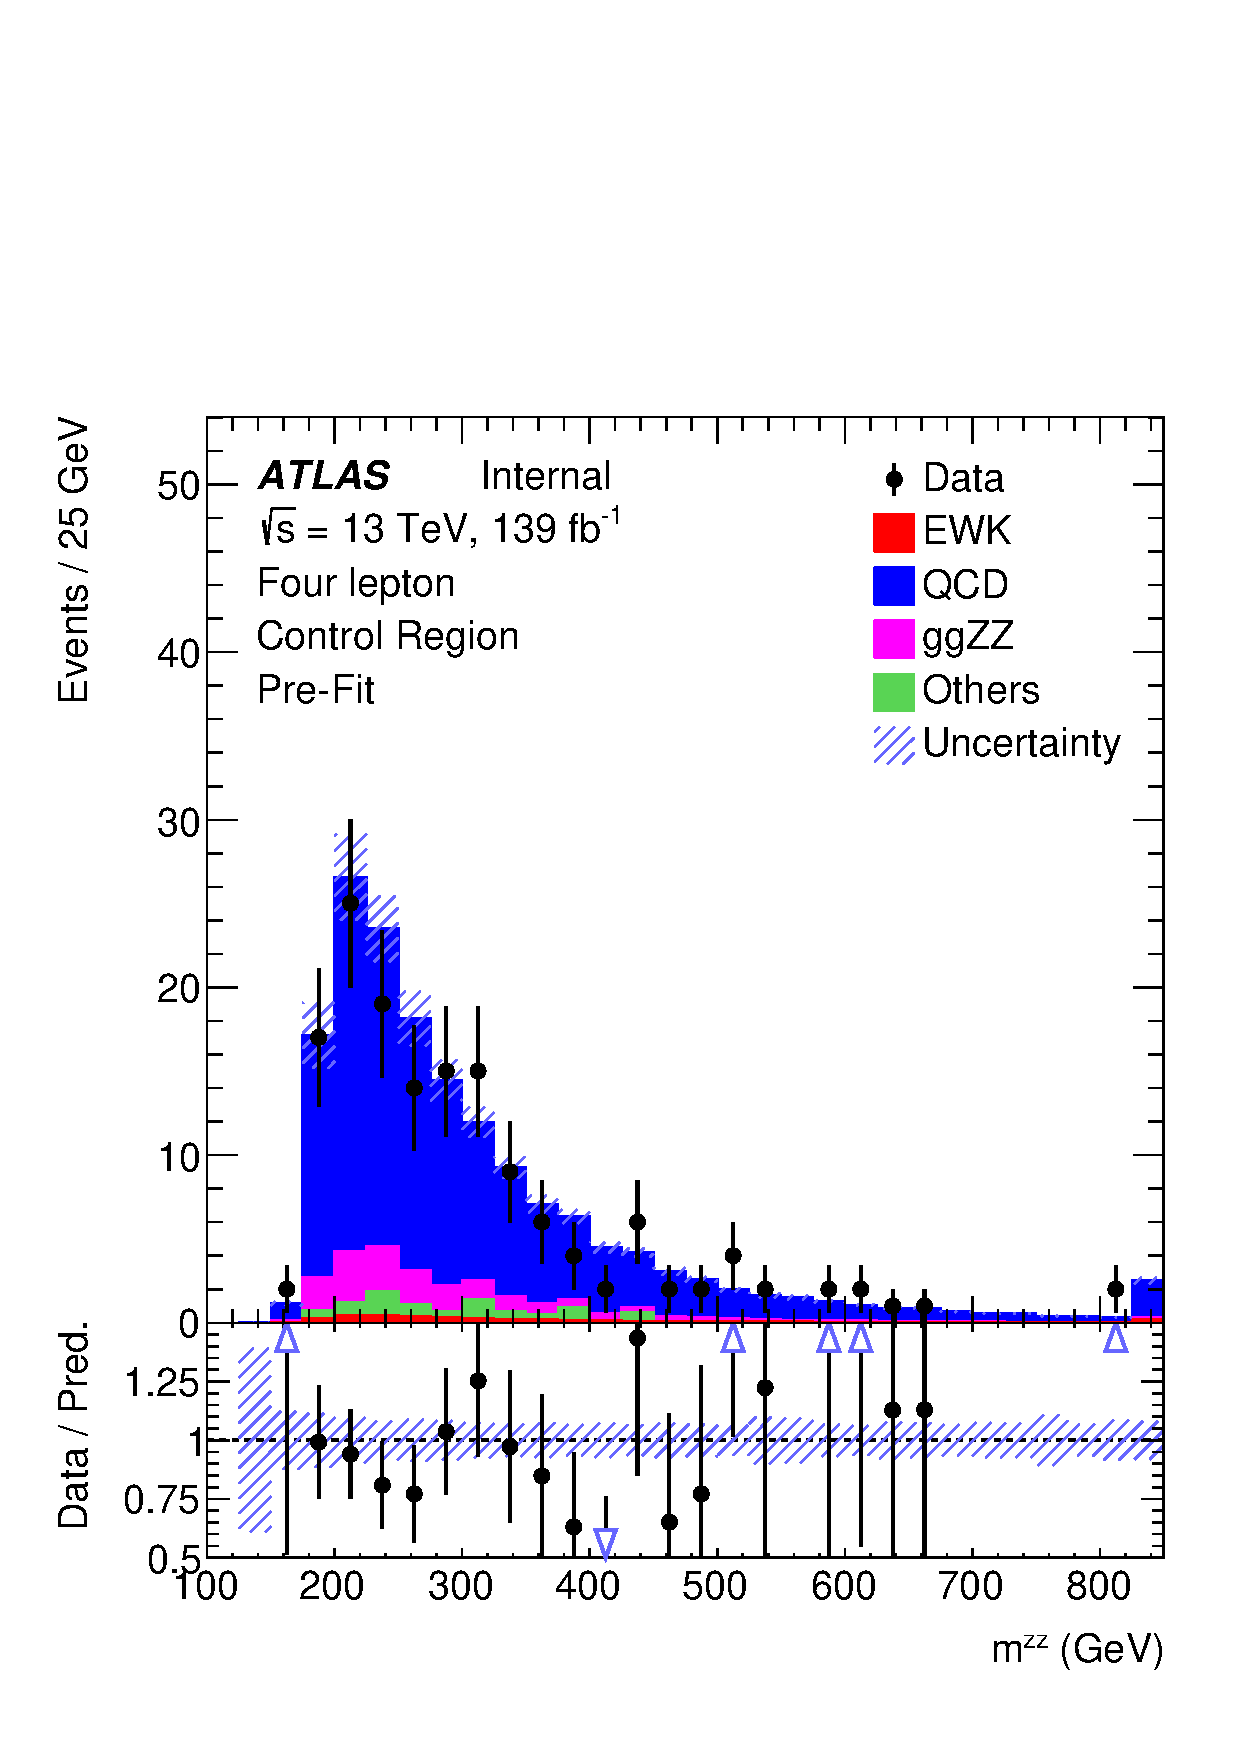
\includegraphics[width=0.42\textwidth]{figures/VBSZZ/QCDCR/MZZ_4l_QCD_CR.pdf}
  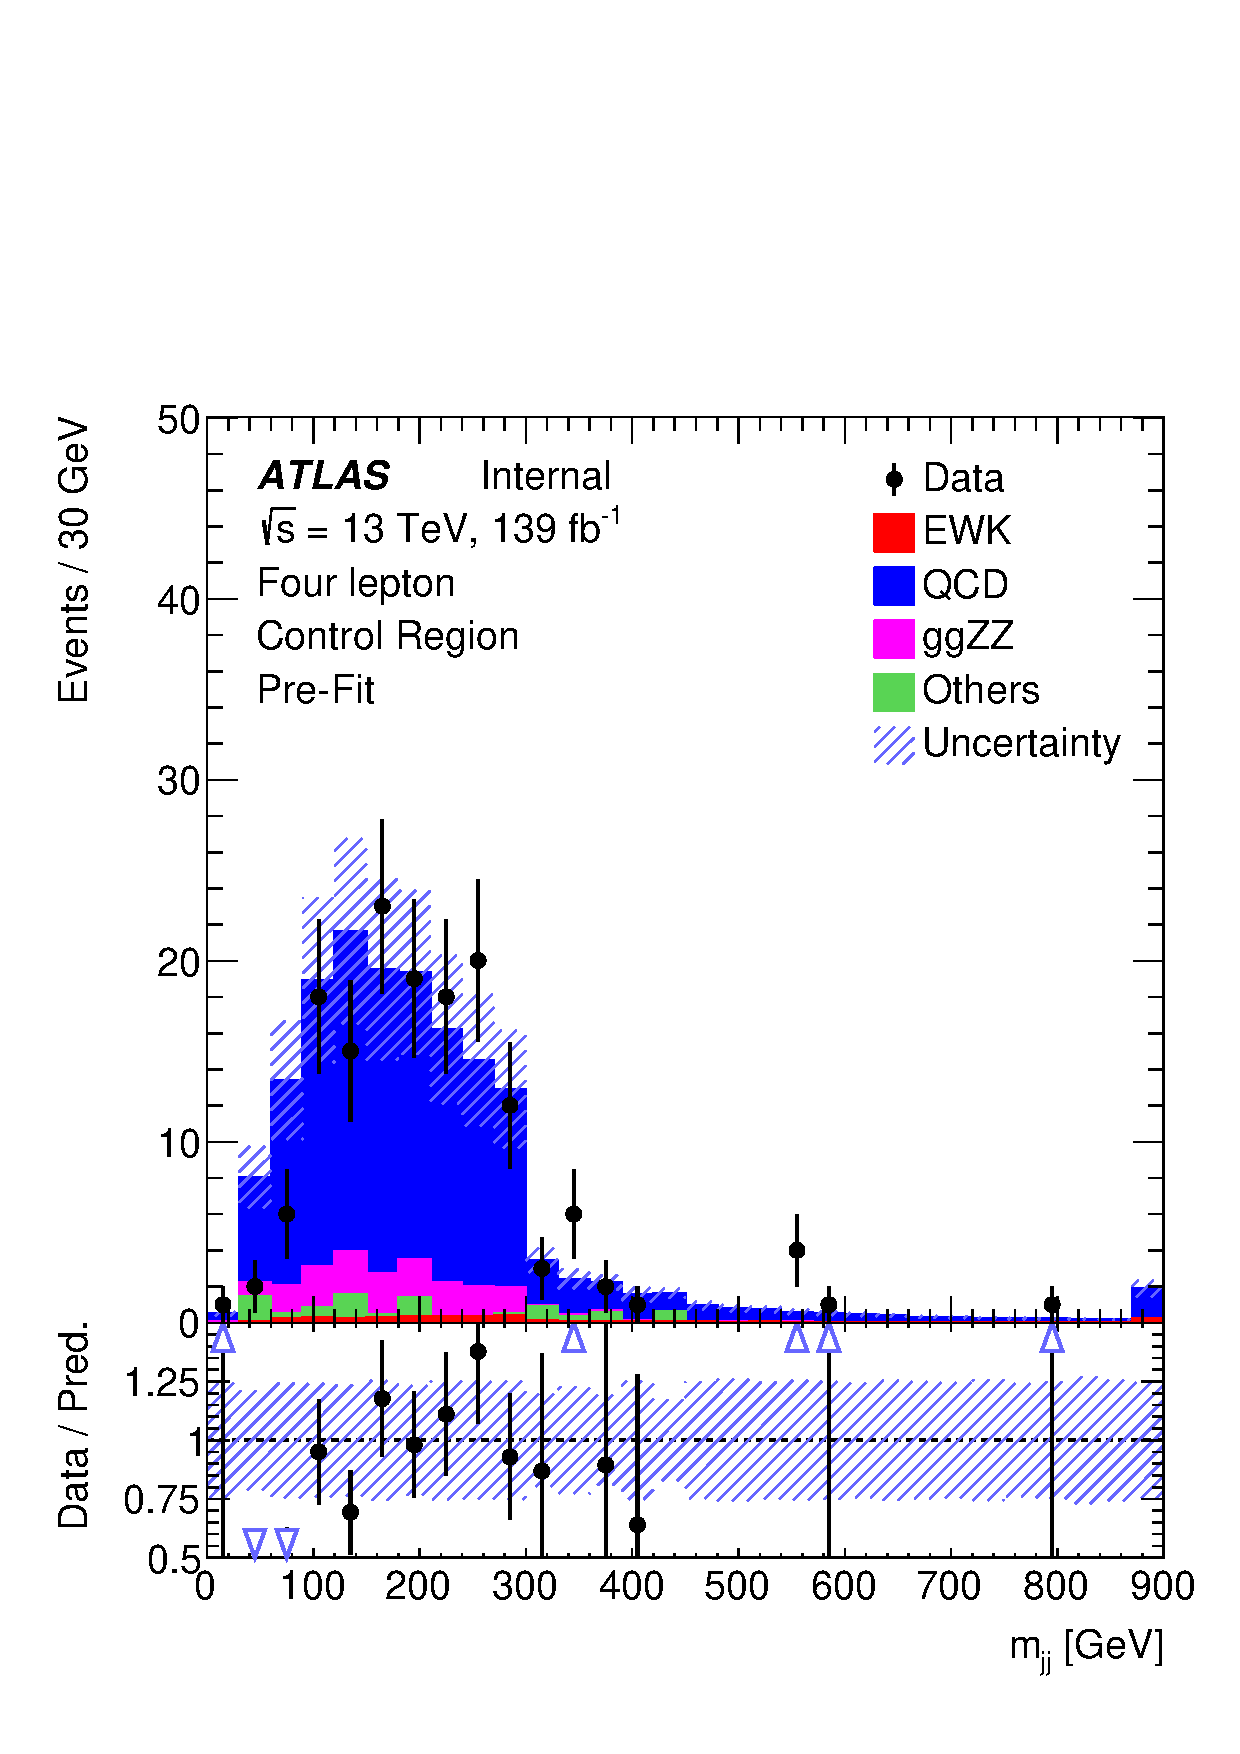
\includegraphics[width=0.42\textwidth]{figures/VBSZZ/QCDCR/MJJ_4l_QCD_CR_fullSyst.pdf}
  \caption{Pre-fit $\mzz$ and $\mjj$ distribution in QCD-enriched CR.}
  \label{fig:qcdcr_prefit}
\end{figure}

\subsection{Fake backgrounds}

Backgrounds from \Zjet, top-quark and $WZ$ processes are estimated by data-driven method.
These events usually contain two or three leptons from Z/W decays, together with heavy-flavor jets or misidentified components of jets reconstructed as leptons called "fake leptons".
A \textit{fake factor} method is used to estimate this backgrounds, in which the lepton misidentification is measured in data regions 
with enhanced contributions from Z + jets and top-quark processes:
\begin{enumerate}
	\item Define a dedicated background dominant region to derive the fake factor for this background. 
The \textit{fake factor} is defined as:
\begin{equation}
	\mathcal{F} = \mathcal{N}_{good} / \mathcal{N}_{pool}
\end{equation}
where $\mathcal{N}_{good}$ refers to the number of good leptons passing all SR selection, while $\mathcal{N}_{pool}$ denotes the number of poor leptons passing most SR selection but fail one certain requirement.
	\item Define a \lllljj fake control region, where one or two leptons pass \textit{poor} requirement while all the other leptons are required to have SR selection.
	\item The number of fake events are calculated as:
\begin{equation}
	\mathcal{N}_{fake} = \left( N_{gggp} - N_{gggp}^{ZZ} \right) \times \mathcal{F} - \left( N_{ggpp} - N_{ggpp}^{ZZ} \right) \times \mathcal{F}^{2}
\end{equation}
with the subtraction of ZZ contribution, and the double counting between ($N_{gggp}$ and $N_{ggpp}$).
\end{enumerate}

For the defination of \textit{poor} leptons:
The poor electrons are defined as failing "FixedCutLoose" isolation requirement or "LooseLH" electron ID requirement but satisfying "VeryLooseLH" WP.
The poor muons are required to fail the "FixedCutLoose" isolation requirement or invert the impact parameter cut to be $3 < d_{0}/\sigma(d_{0}) < 10$.
The dedicated \Zjet and \ttbar dominant regions are defined to calculate the fake factor respectively in the following subsections.
%For other minor fake contributions like $WZ$, $W + jets$ and $W^{+}W^{-} + jets$ without additional dedicated CR, the estimations are included into 

\subsubsection{Fake factor for \Zjet}

Fake factor for \Zjet background is calculated in \Zjet-enriched region, where events with one SFOS lepton pair around Z mass associated with two jets are selected.
The value of fake factor is drived from data, and as a function of $p_{T}$ and $\eta$ as shown in figure~\ref{fig:fake_zjet_el} for electrons and figure~\ref{fig:fake_zjet_mu} for muons.
During calculation, the contributions from non-\Zjet backgrounds (\ttbar, $ZZ$, $WZ$) have been subtracted from data.
The values calculated from \Zjet MC directly are also shown in plots for comparison.
\begin{figure}[!htb]
  \centering
  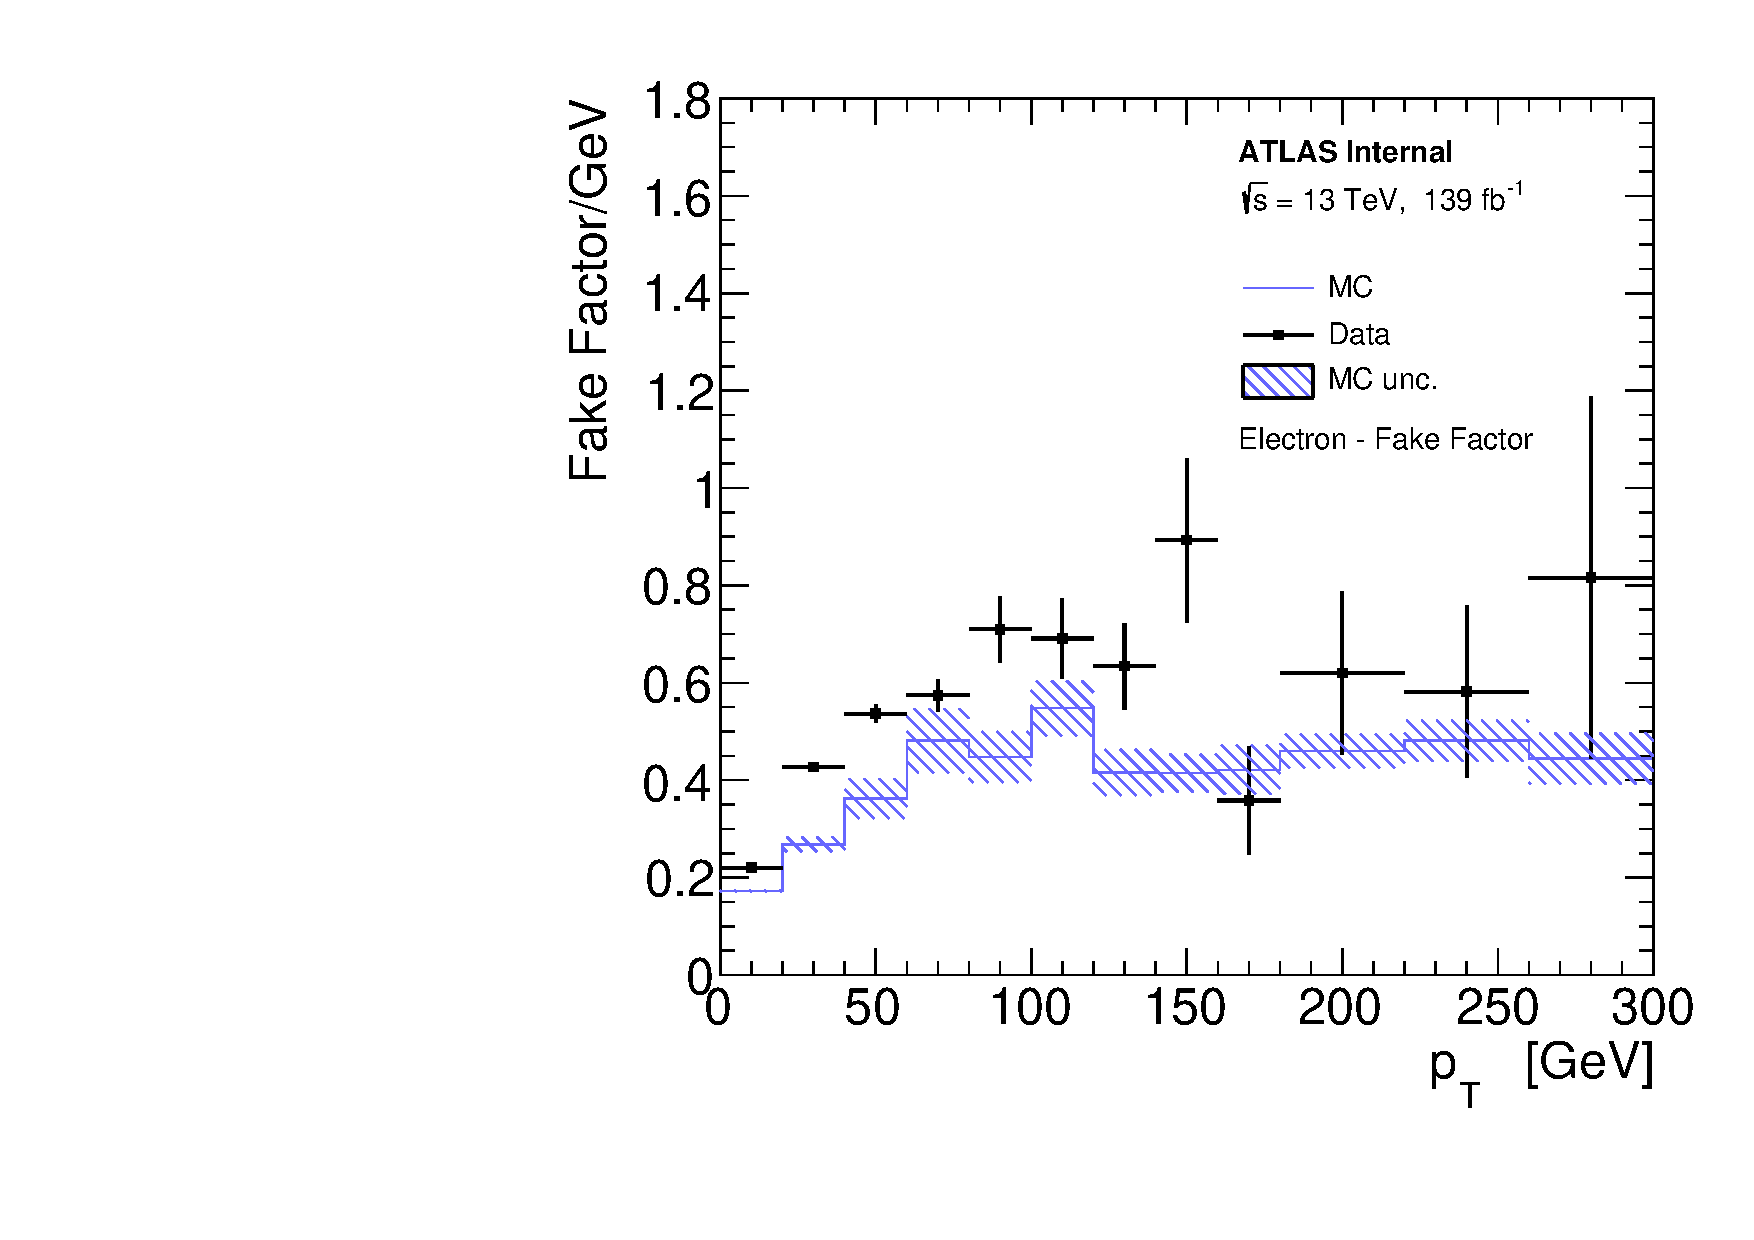
\includegraphics[width=0.42\textwidth]{figures/VBSZZ/fakebkg/Electron_2Dff_ptfakeFactorAddElectron_etapt_pavgy.pdf}
  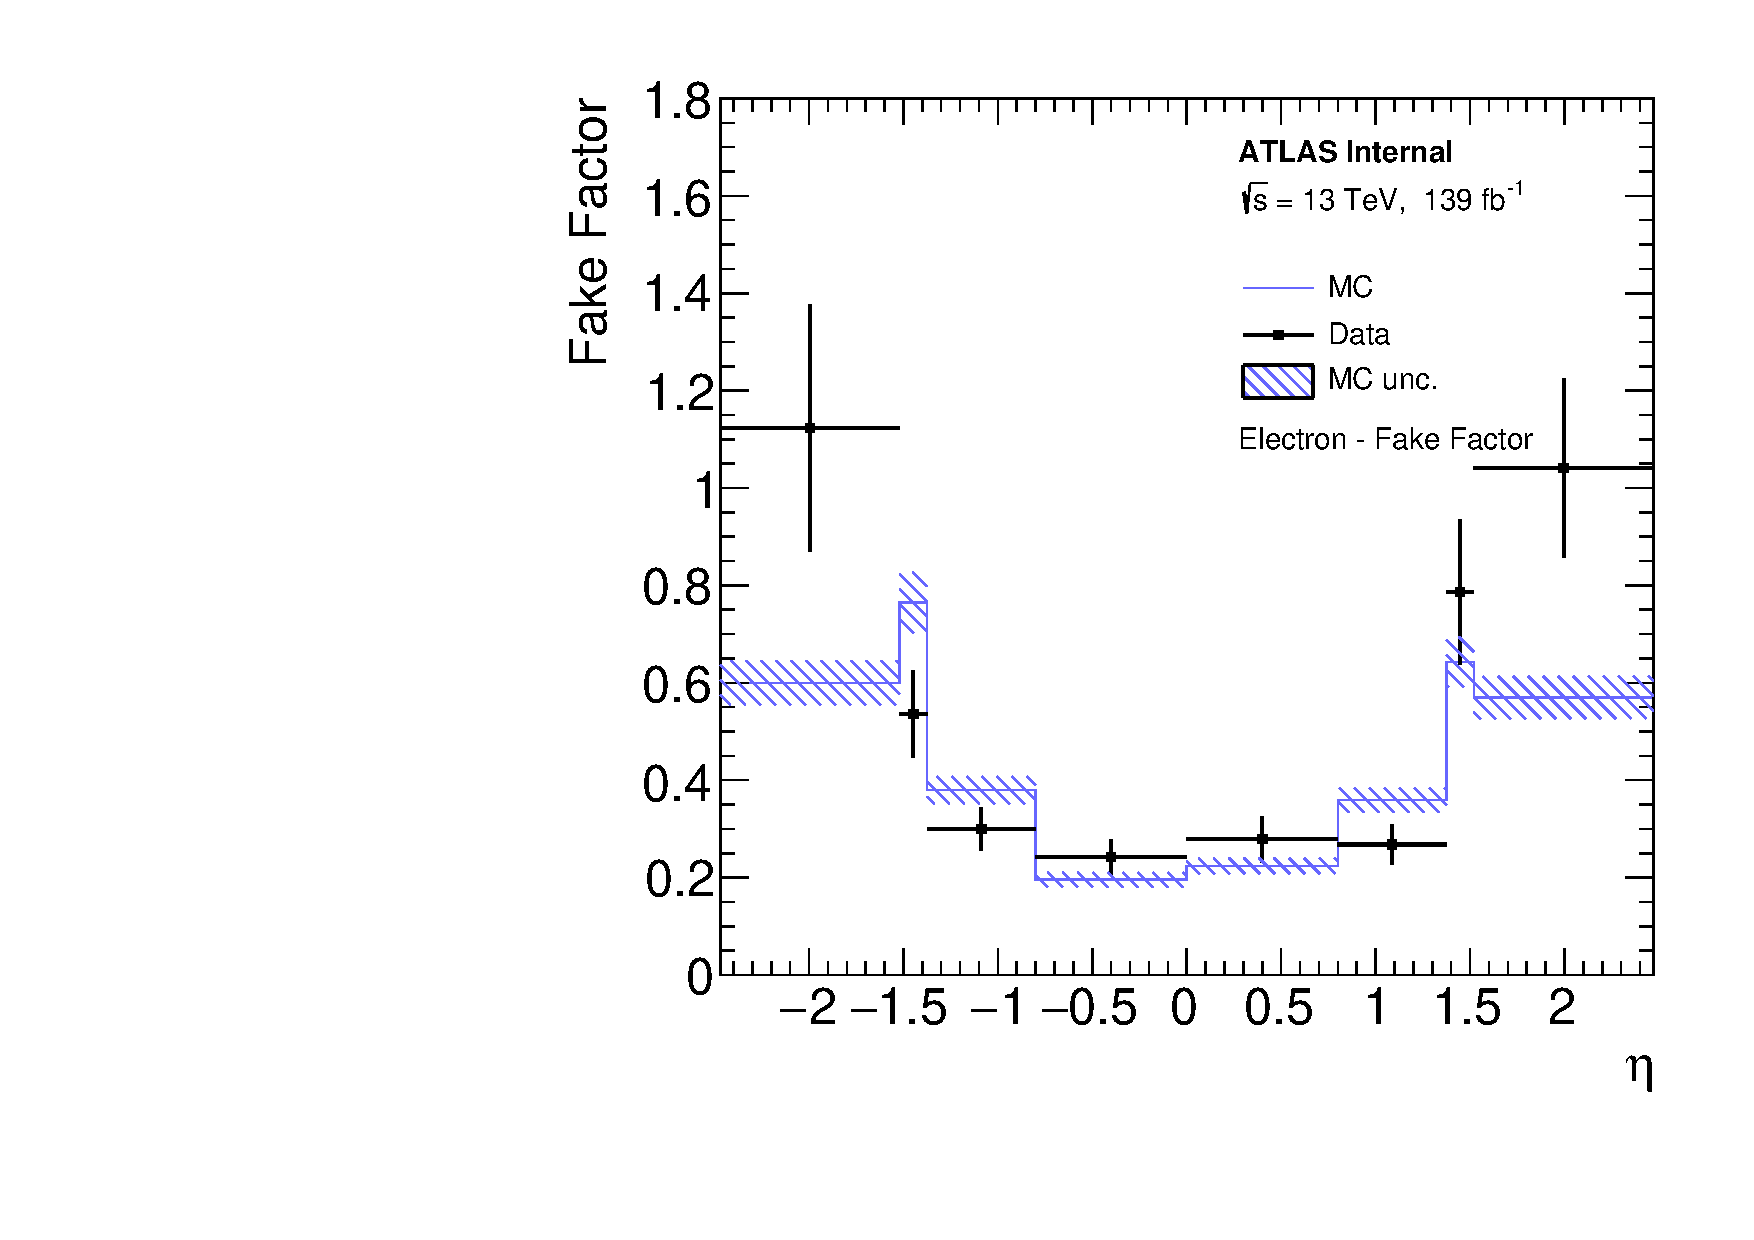
\includegraphics[width=0.42\textwidth]{figures/VBSZZ/fakebkg/Electron_2Dff_etafakeFactorAddElectron_etapt_pavgx.pdf}
  \caption{Fake factor for $\Zjet$ background, constructed with additional electron, as a function of $p_{T}$ (left) and $\eta$ (right).}
  \label{fig:fake_zjet_el}
\end{figure}

\begin{figure}[!htb]
  \centering
  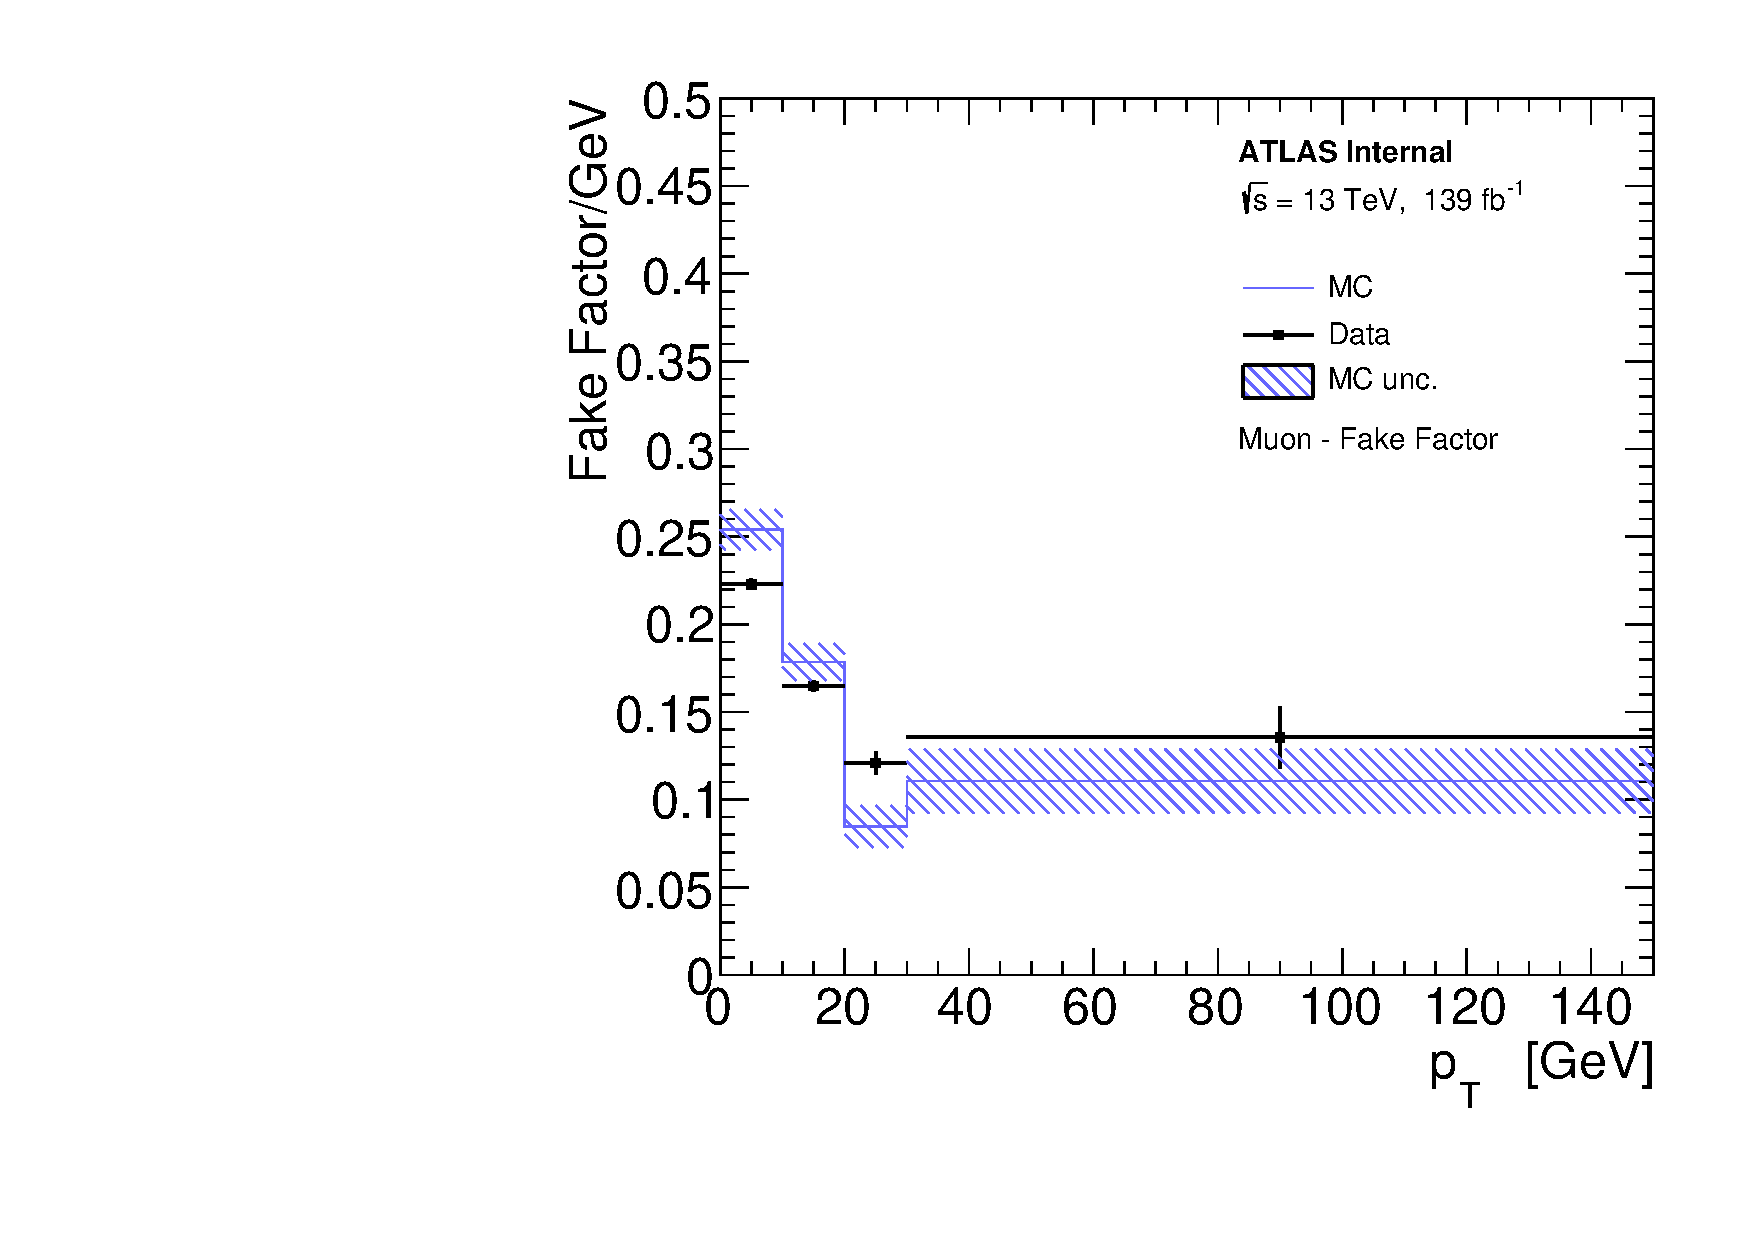
\includegraphics[width=0.42\textwidth]{figures/VBSZZ/fakebkg/Muon_2Dff_ptfakeFactorAddMuon_etapt_pavgy.pdf}
  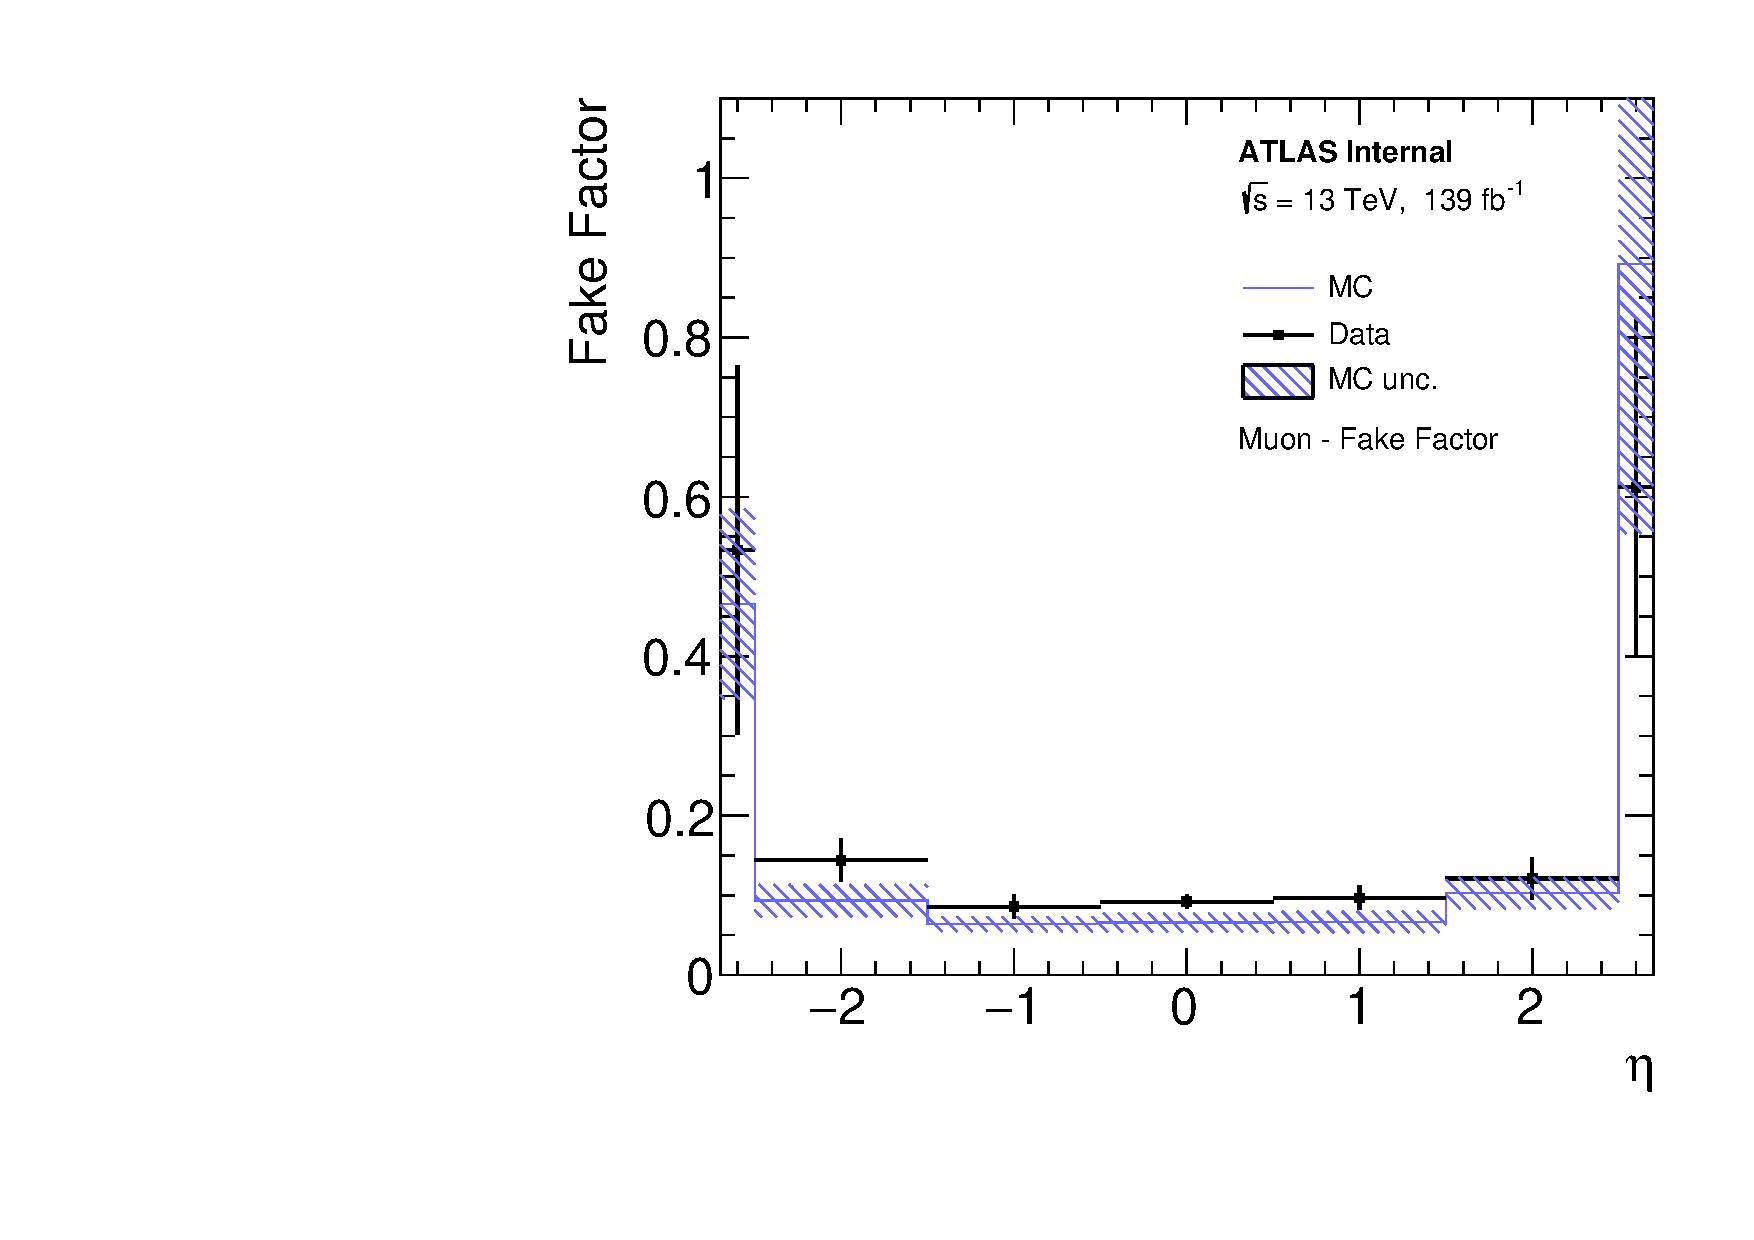
\includegraphics[width=0.42\textwidth]{figures/VBSZZ/fakebkg/Muon_2Dff_etafakeFactorAddMuon_etapt_pavgx.pdf}
  \caption{Fake factor for $\Zjet$ background, constructed with additional muon, as a function of $p_{T}$ (left) and $\eta$ (right).}
  \label{fig:fake_zjet_mu}
\end{figure}

\subsubsection{Fake factor for \ttbar}

The fake factor for \ttbar are calculated in \ttbar dominanted region by selecting one $e\mu$-pair with additional two jets.
For events with three leptons, $m_{T}^{W} <$ 60~\gev cut is applied to reject the constribution from \ttbar + W events.
The $m_{T}^{W}$ is defined as below:
\begin{equation}
	m_{T}^{W} = \sqrt{ 2p_{T}^{l_{3}} E_{T}^{miss} \left[1-cos\left(\Delta\phi\left(p_{T}^{l_{3}}, E_{T}^{miss}\right)\right)\right] }
\end{equation}
In addition, at least one b-jet is required to enhance the top component.
The fake factors of \ttbar calculated from data as the function of $p_{T}$ and $\eta$ are shown in figure~\ref{fig:fake_tt_el} for electrons and ~\ref{fig:fake_tt_mu} for muons.
The non-\ttbar contributions, which include \Zjet, $ZZ$ and $WZ$, are subtracted from data.
\begin{figure}[!htb]
  \centering
  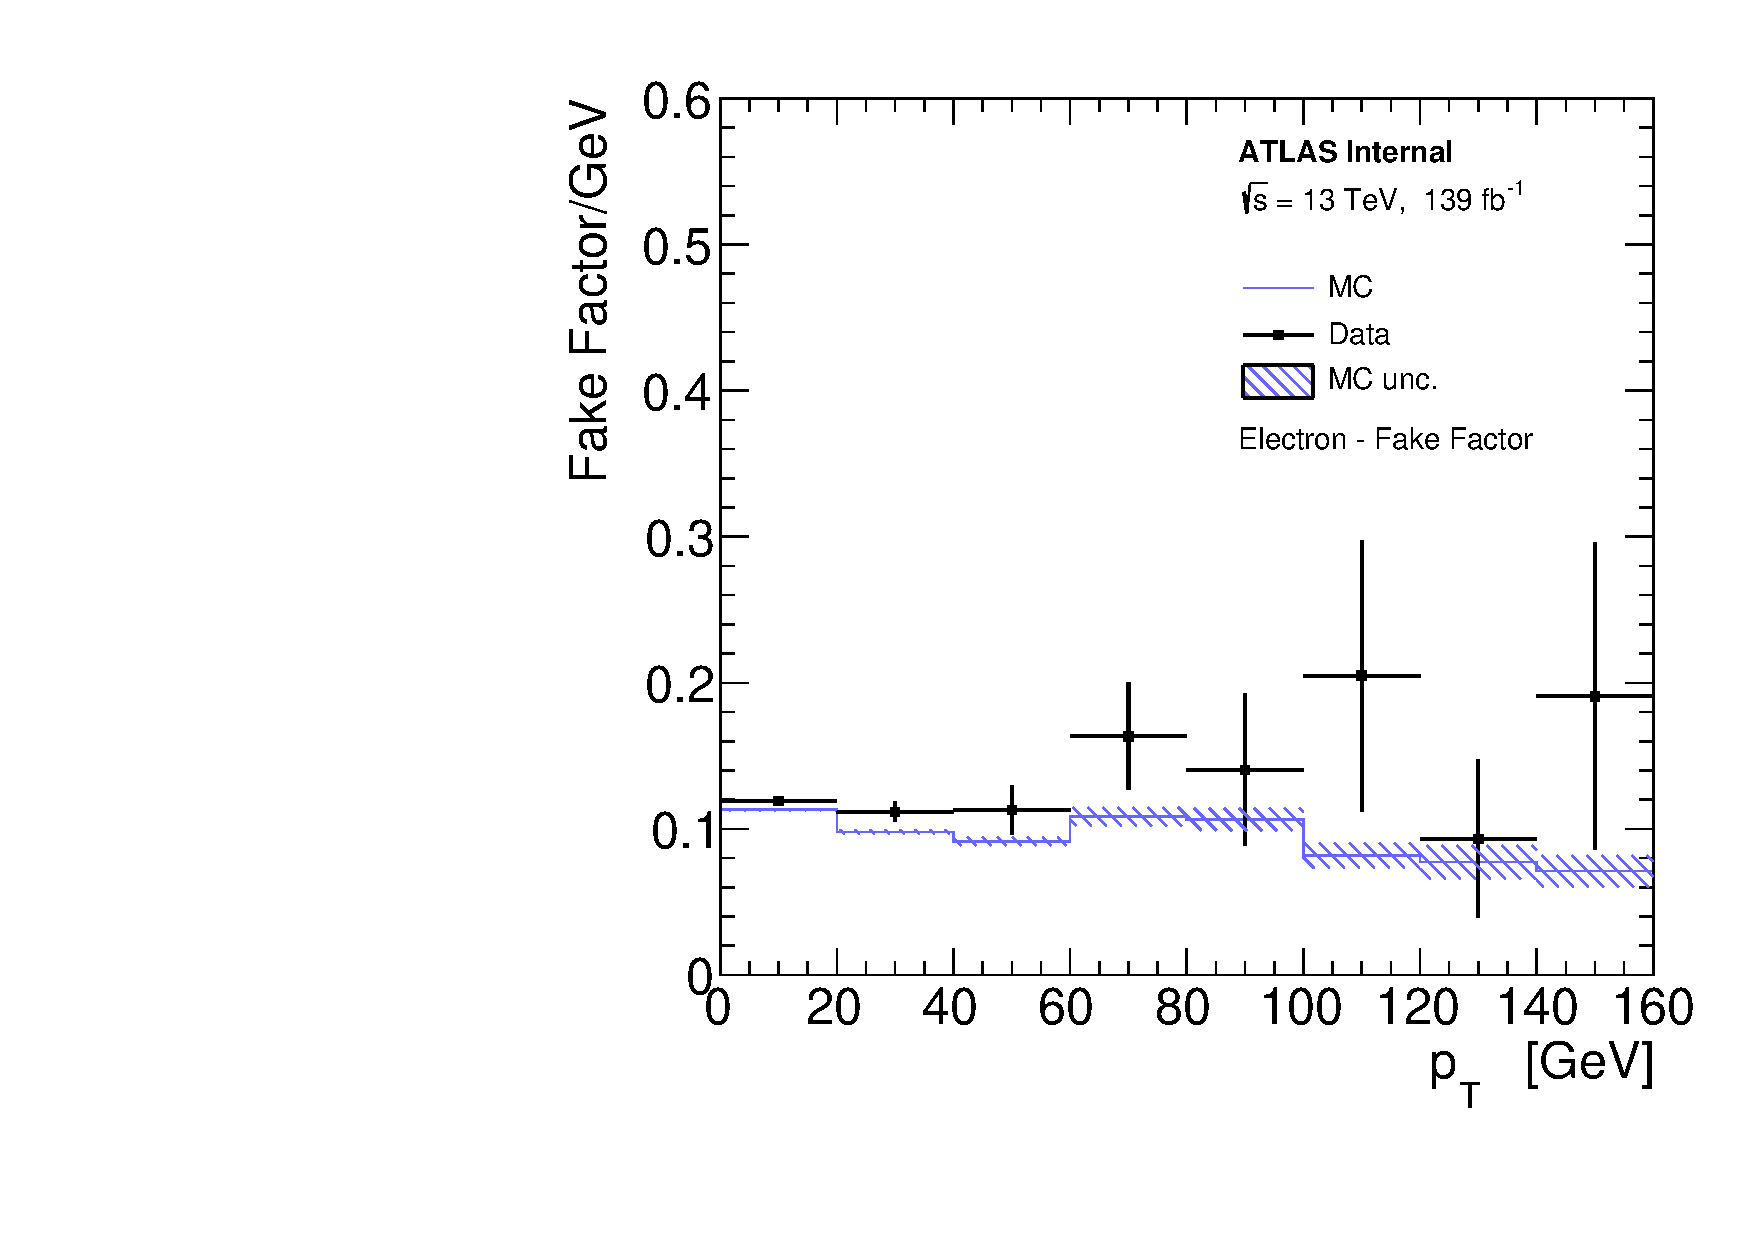
\includegraphics[width=0.42\textwidth]{figures/VBSZZ/fakebkg/Electron_2Dff_ptttbarFakeFactorAddElectron_etapt_pavgy.pdf}
  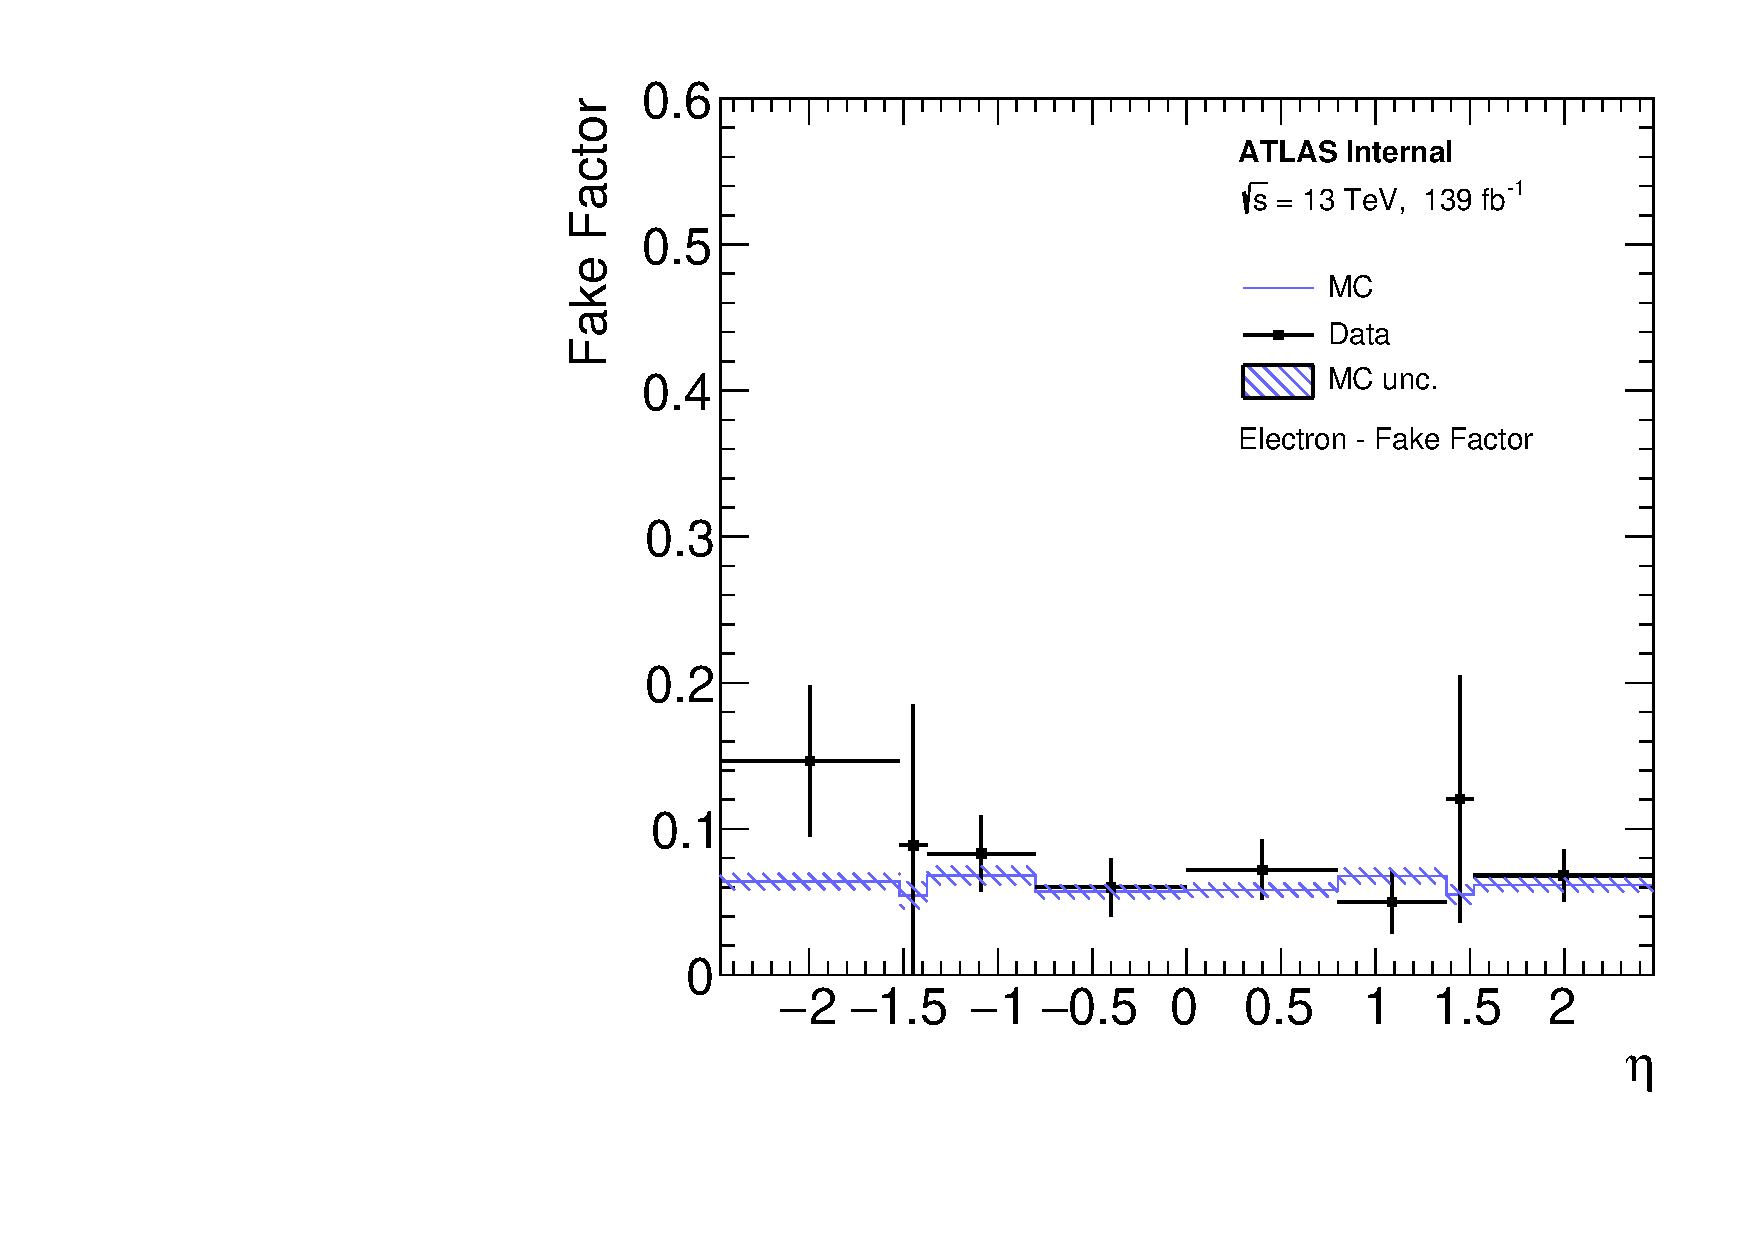
\includegraphics[width=0.42\textwidth]{figures/VBSZZ/fakebkg/Electron_2Dff_etattbarFakeFactorAddElectron_etapt_pavgx.pdf}
  \caption{Fake factor for $\ttbar$ background, constructed with additional electron, as a function of $p_{T}$ (left) and $\eta$ (right).}
  \label{fig:fake_tt_el}
\end{figure}

\begin{figure}[!htb]
  \centering
  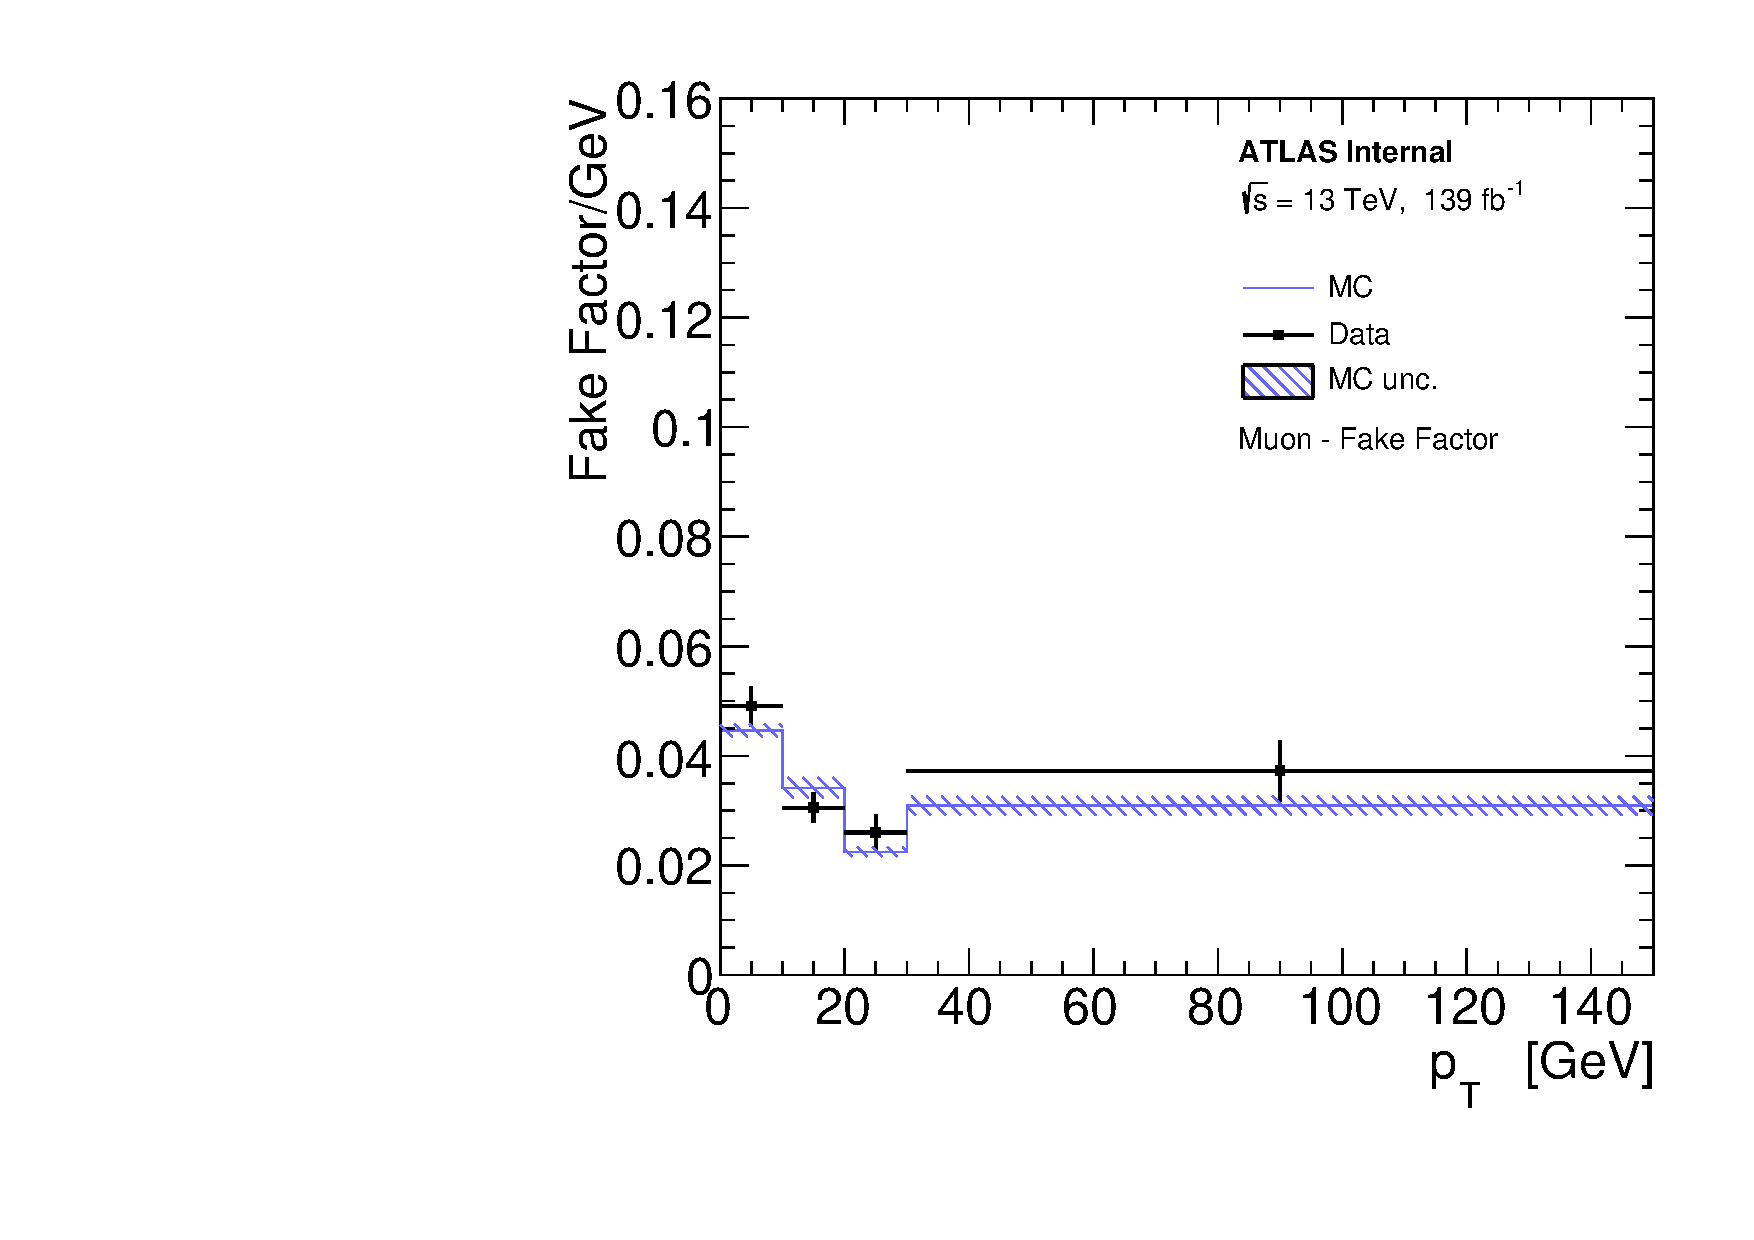
\includegraphics[width=0.42\textwidth]{figures/VBSZZ/fakebkg/Muon_2Dff_ptttbarFakeFactorAddMuon_etapt_pavgy.pdf}
  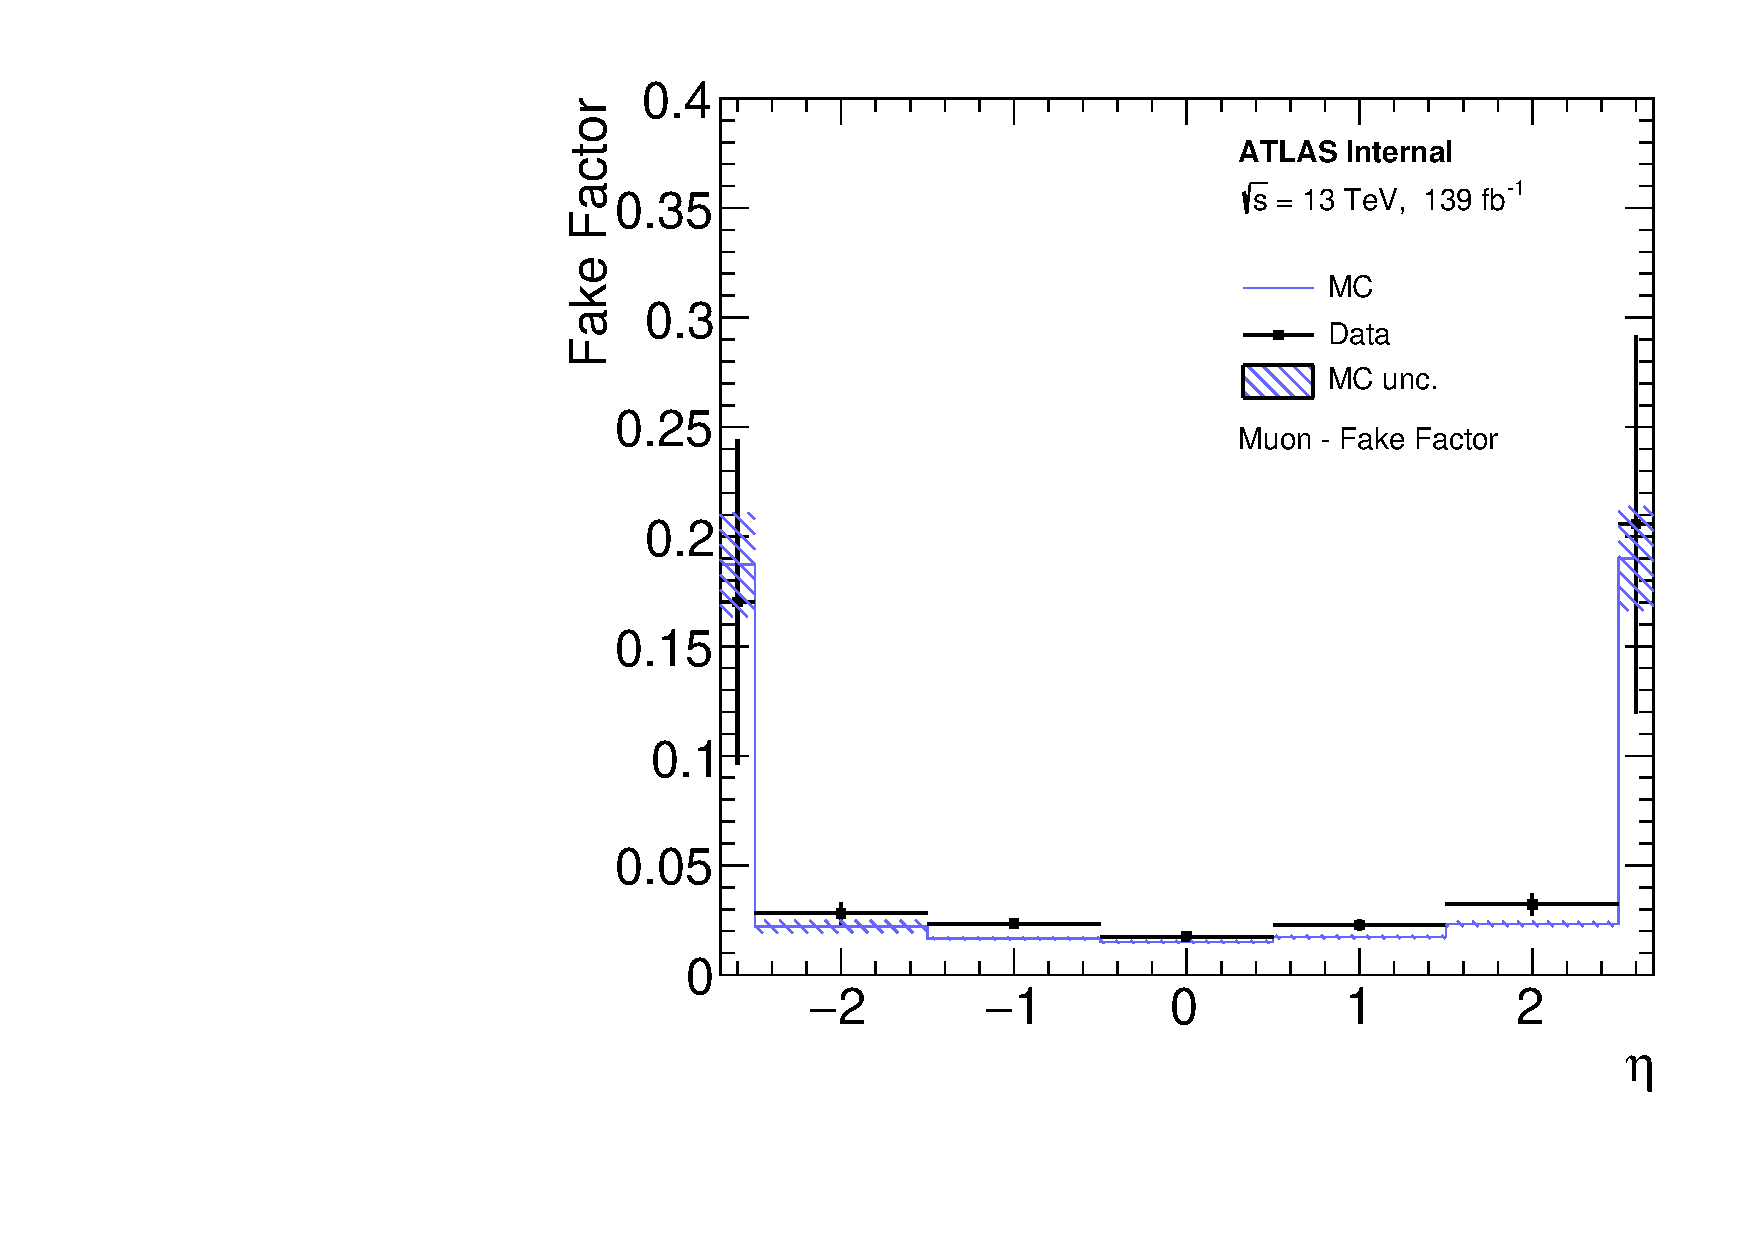
\includegraphics[width=0.42\textwidth]{figures/VBSZZ/fakebkg/Muon_2Dff_etattbarFakeFactorAddMuon_etapt_pavgx.pdf}
  \caption{Fake factor for $\ttbar$ background, constructed with additional muon, as a function of $p_{T}$ (left) and $\eta$ (right).}
  \label{fig:fake_tt_mu}
\end{figure}

\subsubsection{Combination}

The fake factors calculated from each dedicated region are then combined together according to their contributions in fake control region described previously.
Figure~\ref{fig:fake_mjj} shows the \mjj distribution with data and major fake backgrounds in three different 4l channels.
\begin{figure}[!htb]
  \centering
  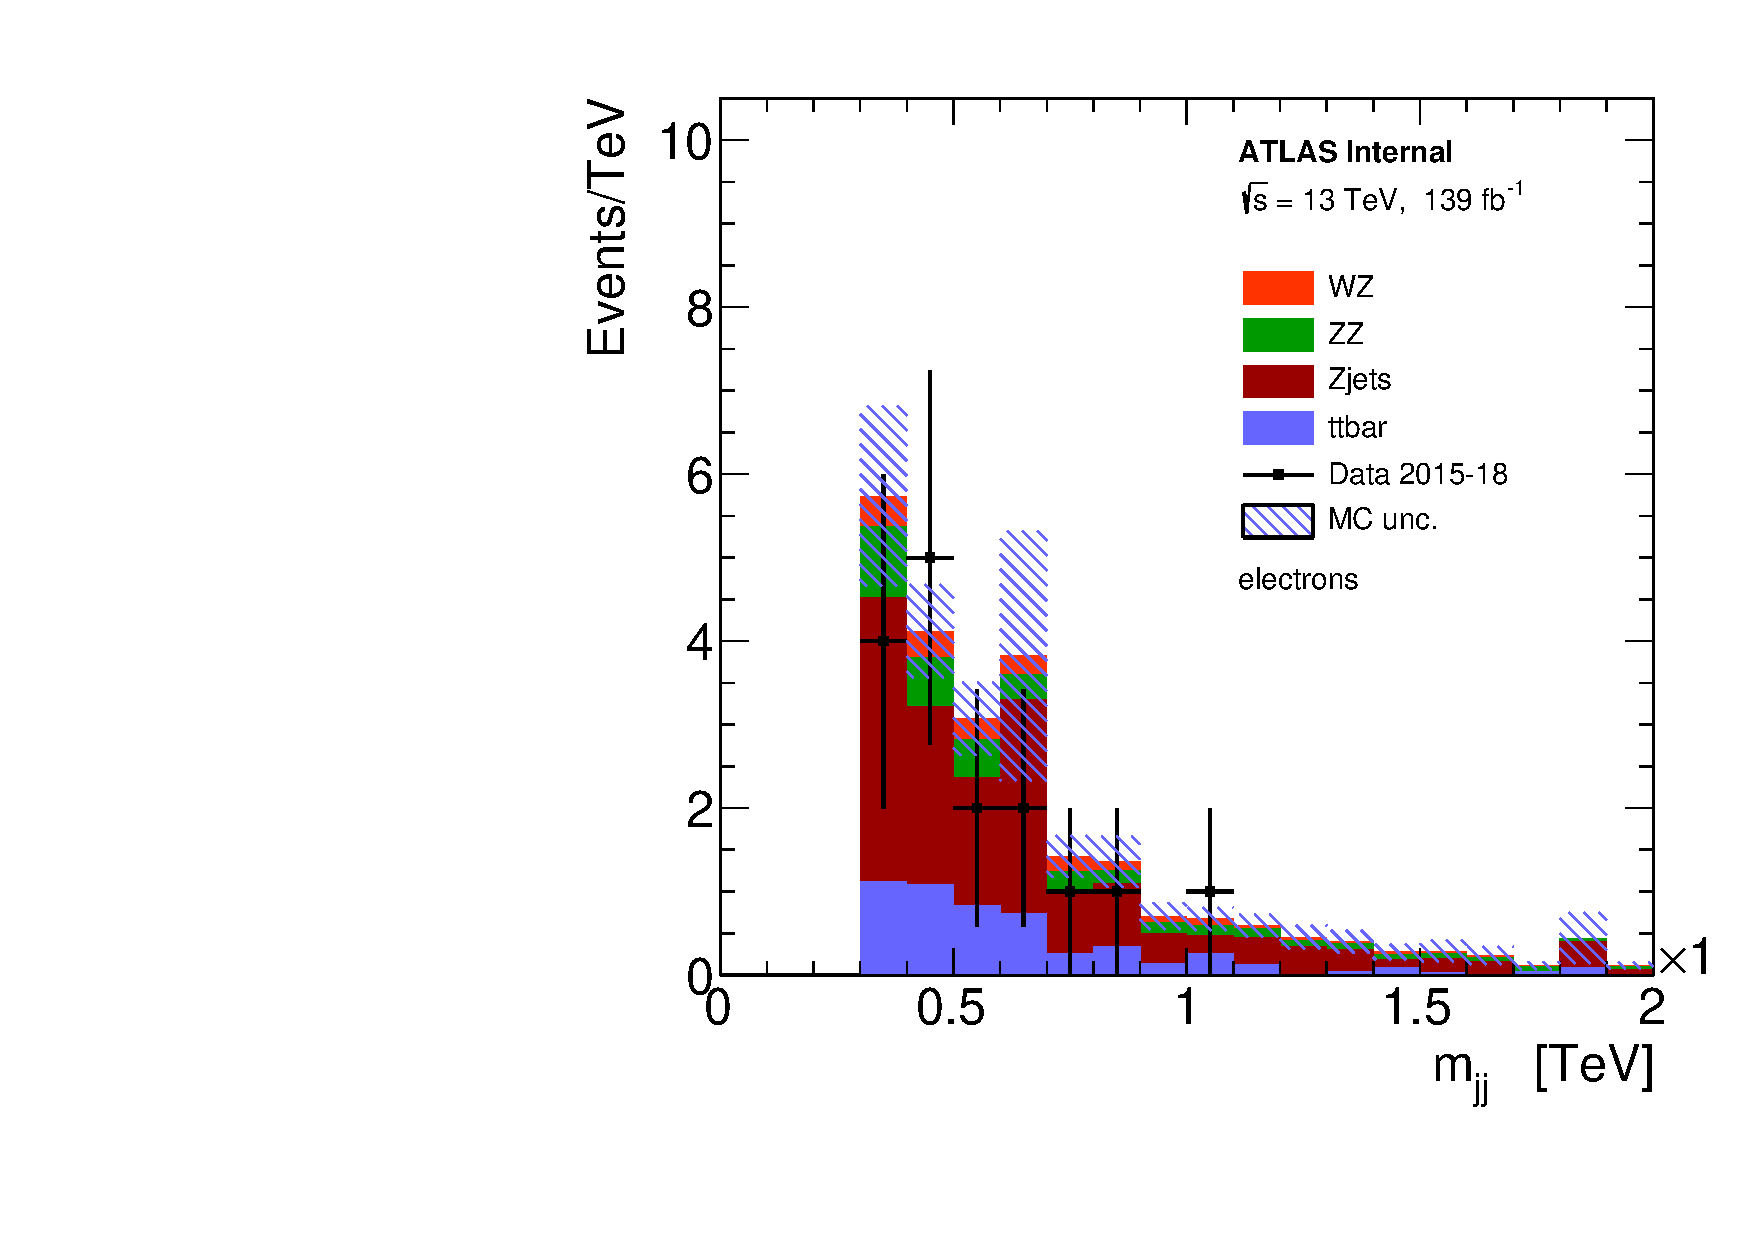
\includegraphics[width=0.32\textwidth]{figures/VBSZZ/fakebkg/15161718_mva_dijet_mass_zjet_ttbar_ratio_electrons_mva_dijet_mass.pdf}
  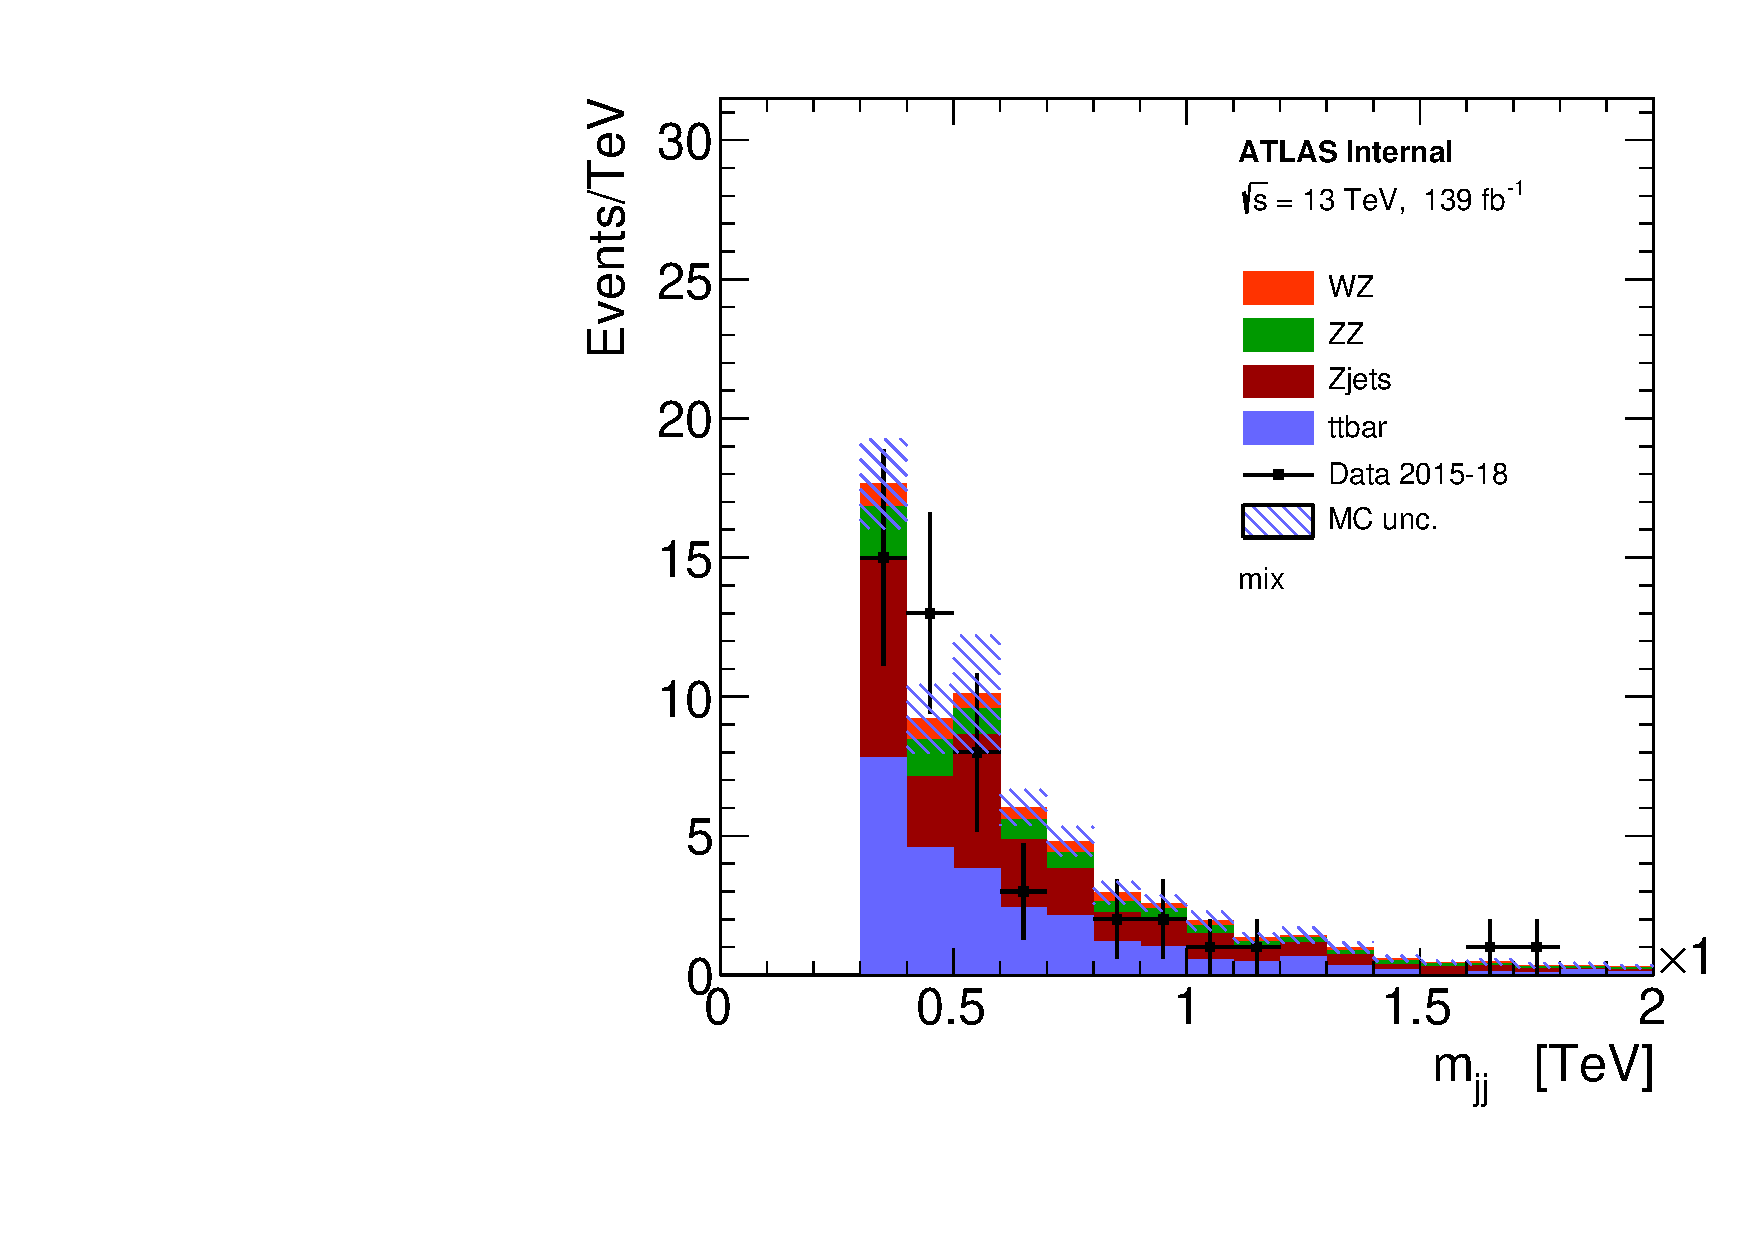
\includegraphics[width=0.32\textwidth]{figures/VBSZZ/fakebkg/15161718_mva_dijet_mass_zjet_ttbar_ratio_mix_mva_dijet_mass.pdf}
  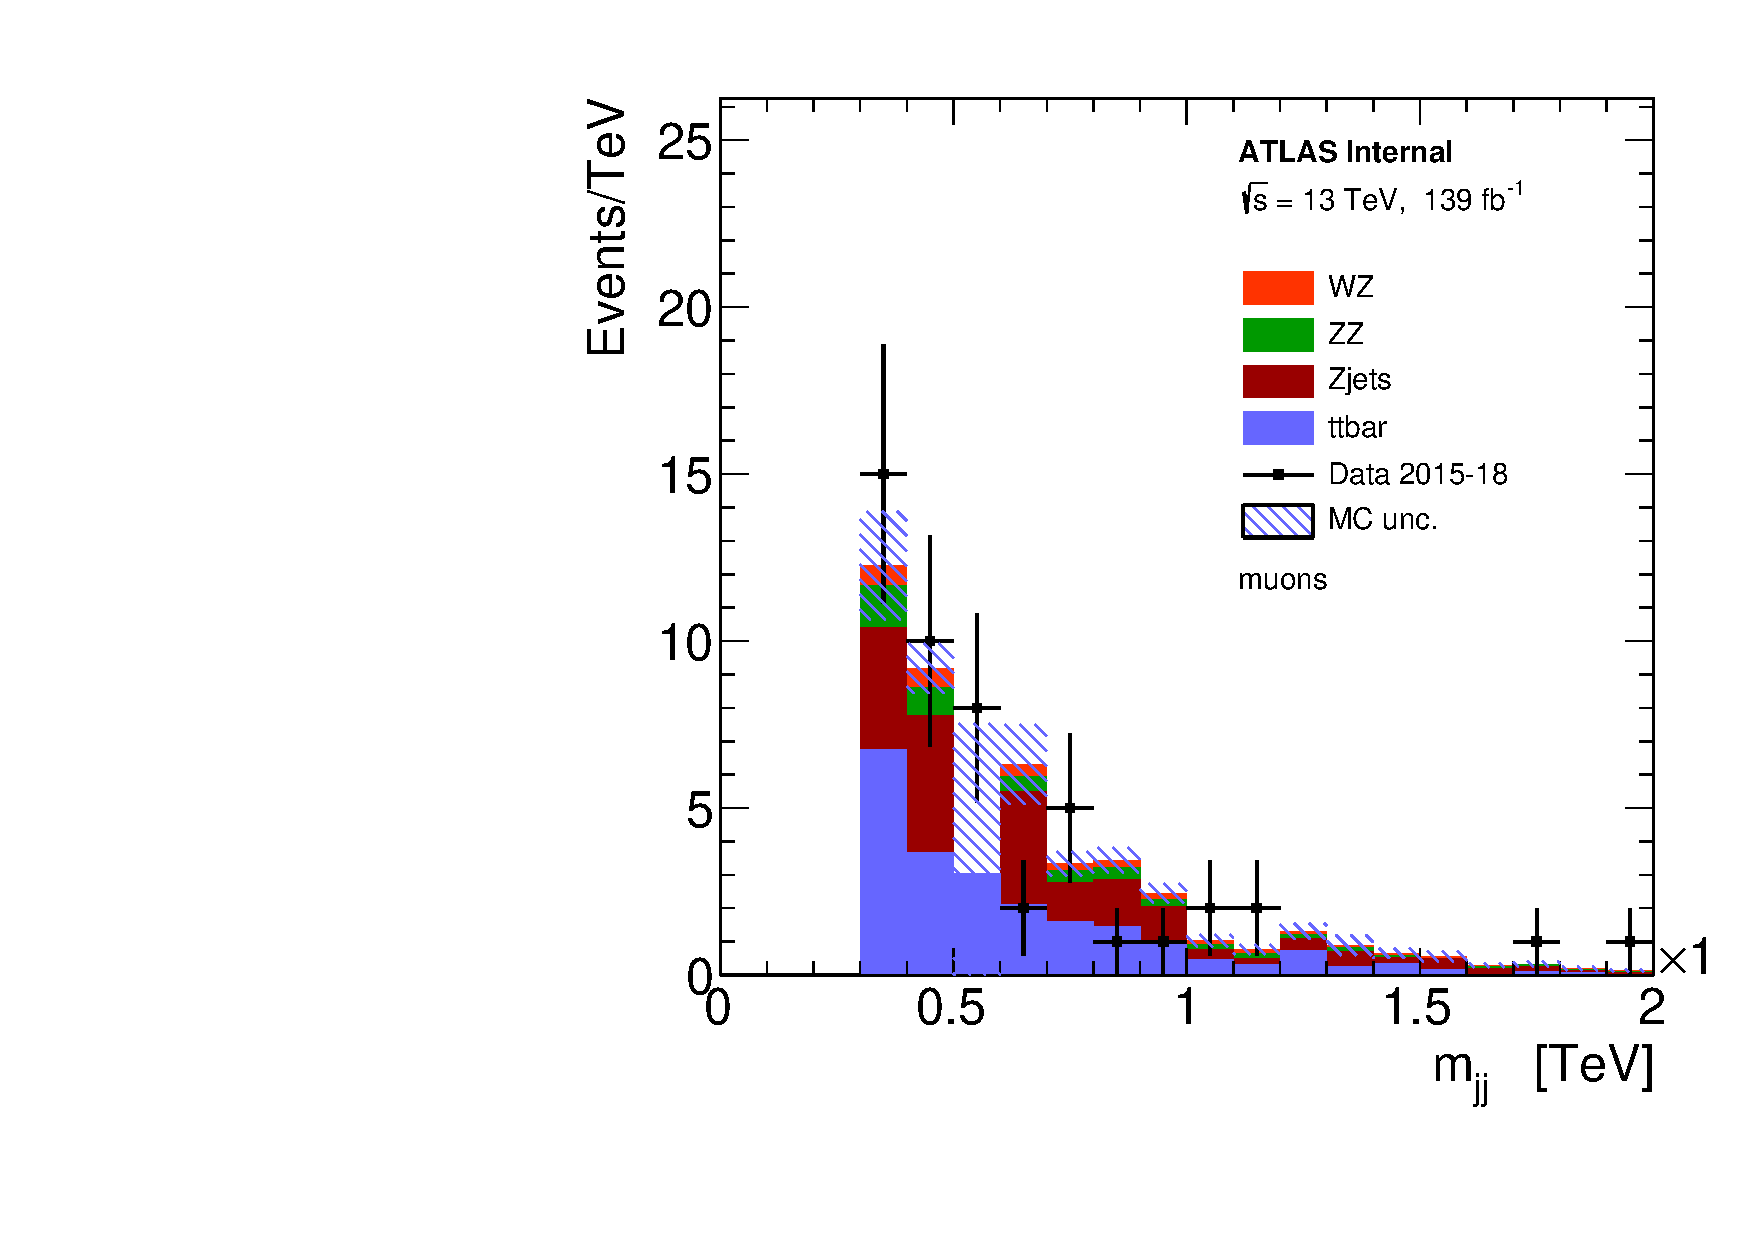
\includegraphics[width=0.32\textwidth]{figures/VBSZZ/fakebkg/15161718_mva_dijet_mass_zjet_ttbar_ratio_muons_mva_dijet_mass.pdf}
  \caption{$\mjj$ distributions in fake control region in 4e (left), 2e2$\mu$ (middle) and 4$\mu$ (right) channel.
The ratios between $\Zjet$ and $\ttbar$ ($\Zjet / \ttbar$) in each individual channel are: 2.59, 0.95, 0.74.}
  \label{fig:fake_mjj}
\end{figure}

\subsubsection{Systematics of fake estimation and results}
\label{sec:fake_syst}

The systematics of fake factor method can be measured by varying the parameters and selection requirements in fake factor calculation.
In addition, due to the very limited data statistic in \llll channel, to be more conservative, 
the difference between data measurement and MC simulation are also considered as another systematics component.
In detail, the sources of systematics that have been included are listed as follow:
\begin{itemize}
	\item Variation of isolation cut for the poor lepton definition up and down scaled by factor of two.
	\item Variation of the yield of those subtracted MC in fake control region by 30\% up and down.
	\item The difference of fake factors between drived from data and from MC simulation.
	\item The difference of fake factors when changing to one bin measurement (instead of $p_{T}$ ot $\eta$ dependent).
	\item The statistical uncertainties on fake factor in fake control region.
\end{itemize}

Table~\ref{tab:fake_uncer} summarizes the contribution of fake backgrounds in signal region under different systematic conditions mentioned above as well as the nominal one.
Uncertainties of each value in table are statistical one.
\begin{table}[h]
    \centering
    \resizebox{1.0\columnwidth}{!}{
        \begin{tabular}{lrrrr}
        channel & 4e &   2e2$\mu$ &    4$\mu$ &   inclusive \\ 
	\hline
        Nominal estimate                  & 0.678$\pm$ 0.652 & 1.023$\pm$ 0.740 & 0.566$\pm$ 0.240 & 2.268$\pm$ 1.015 \\
        $F$ stat. uncertainty varied down & 0.698$\pm$ 0.622 & 0.872$\pm$ 0.652 & 0.509$\pm$ 0.214 & 2.079$\pm$ 0.926 \\
        $F$ stat. uncertainty varied up   & 0.657$\pm$ 0.685 & 1.173$\pm$ 0.840 & 0.622$\pm$ 0.267 & 2.452$\pm$ 1.116 \\
        One bin $F$                       & 0.653$\pm$ 0.590 & 0.594$\pm$ 0.558 & 0.646$\pm$ 0.313 & 1.892$\pm$ 0.870 \\
        MC $F$                            & 0.534$\pm$ 0.471 & 1.415$\pm$ 0.993 & 0.439$\pm$ 0.184 & 2.389$\pm$ 1.114 \\
        Isolation varied down             & 0.938$\pm$ 0.686 & 0.552$\pm$ 0.466 & 0.215$\pm$ 0.107 & 1.704$\pm$ 0.837 \\
        Isolation varied up               & 0.723$\pm$ 0.646 & 1.104$\pm$ 0.739 & 0.559$\pm$ 0.237 & 2.386$\pm$ 1.010 \\
        MC corr. varied down              & 0.697$\pm$ 0.695 & 1.048$\pm$ 0.811 & 0.832$\pm$ 0.385 & 2.577$\pm$ 1.136 \\
        MC corr. varied up                & 0.660$\pm$ 0.614 & 0.984$\pm$ 0.687 & 0.316$\pm$ 0.159 & 1.961$\pm$ 0.935 \\
        \hline
        \end{tabular}
        }
    \caption{
    Fake background estimations in the SR. For the nominal value the 2D fake factor together with the $Z$+jets and $t\bar{t}$ combination is applied.
    The other lines show the estimatins with different uncertainty variations.
    }
    \label{tab:fake_uncer}
\end{table}

